%%%%%%%% ICML 2021 EXAMPLE LATEX SUBMISSION FILE %%%%%%%%%%%%%%%%%

\documentclass{article}

% Recommended, but optional, packages for figures and better typesetting:
\usepackage{microtype}
\usepackage{graphicx}
\usepackage{amssymb}
\usepackage{color}
\usepackage[font=footnotesize,labelfont=bf]{caption}
\usepackage[square,numbers]{natbib}
\usepackage[margin=1in]{geometry}
\usepackage{subfigure}
\usepackage{booktabs} % for professional tables
\bibliographystyle{unsrtnat}

% hyperref makes hyperlinks in the resulting PDF.
% If your build breaks (sometimes temporarily if a hyperlink spans a page)
% please comment out the following usepackage line and replace
% \usepackage{icml2021} with \usepackage[nohyperref]{icml2021} above.
\usepackage{hyperref}

% Attempt to make hyperref and algorithmic work together better:
\newcommand{\theHalgorithm}{\arabic{algorithm}}

% Use the following line for the initial blind version submitted for review:
%\usepackage{icml2021}

% If accepted, instead use the following line for the camera-ready submission:
%\usepackage[accepted]{icml2021}

% The \icmltitle you define below is probably too long as a header.
% Therefore, a short form for the running title is supplied here:
% \icmltitlerunning{Submission and Formatting Instructions for ICML 2021}

\begin{document}

\twocolumn[\centering\Large{\textbf{Parallel Implementation of Gray Level Co-occurrence Matrix Construction using MPI}}\vspace*{0.75 cm}\\ \normalsize{Aditi Jaiswal, Arianna Bunnell, and Sorapong Khongnawang}\vspace*{1 cm}]


\begin{abstract}

\end{abstract}

\section{Introduction}
    Image texture is an important feature in computer vision tasks. Textural features have been developed to allow for objective comparison of textures between images and image regions. Haralick introduced the Gray-Level Co-Occurrence Matrix (GLCM) in 1973 as a necessary step for the computation of the Haralick texture features \cite{haralick}. Constructing the GLCM for a given grayscale image involves analyzing the spatial relationships between each pixel and its neighbors for a given angle and distance \cite{haralick}. The computation of the GLCM is computationally expensive and its execution time relies heavily on the size of the image. For a grayscale image of size $n \times n$, construction of the GLCM demands $n^2$ memory accesses and $n$ writes. In this paper, we compare several methods for parallel construction of the GLCM using MPI. 
\section{Background}
\subsection{Gray-Level Co-occurrence Matrix}
    Haralick devised the GLCM (referred to as Gray-Tone Spatial-Dependence Matrices in his work) as a preliminary step for the computation of the Haralick textural features \cite{haralick}. The GLCM is a flexible measure of spatial dependence between pixel gray levels which is defined by an angle, a distance, and the unique gray tones in an image. We define the GLCM for some grayscale image $A$, generally following Haralick's notation, below. \\ \\
    Suppose image $A$ has dimensions $n \times m$ pixels. If we suppose the gray level in each pixel lies within the range 0-255. We assume here the image is stored in the standard byte format, with each pixel value stored as an 8-bit integer. We let $N = \{ 1, 2, ..., n\}$ and $M = \{1, 2, ..., m\}$ be the spatial coordinates of the pixels along the vertical and horizontal domains, respectively. Thus, the set $N \times M $ represents all spatial coordinates in the image $A$. Each spatial coordinate maps to a single gray level. We then arrive at the following mapping which defines the gray tones in an image: $ A:  N \times M \to G$, where $G$ is the set of all gray tones. \\
    The GLCM is a matrix of frequencies. We record the frequency that each pair of gray tones $g_e$ and $g_f$ occur within some distance $d$ of each other, at some angle $a$, where $g_e, g_f \in G$, $a \in \{0, 45, 90, 135\}$ and $d \in \{1, 2, ..., \min(m, n)\}$. Thus, GLCM $\in \mathbb{N}^{c \times c}$ where $c$ is the cardinality of the set $G$ for our given image $A$. The angle $a$ defines along which axis we walk the distance $d$ and is pictured in Figure \ref{fig:directions}. Each pixel $p$ in an image then has 8 possible neighboring pixels, excluding those for which these neighbors would extend beyond the edge of the grayscale image $A$. 
    \begin{figure}
      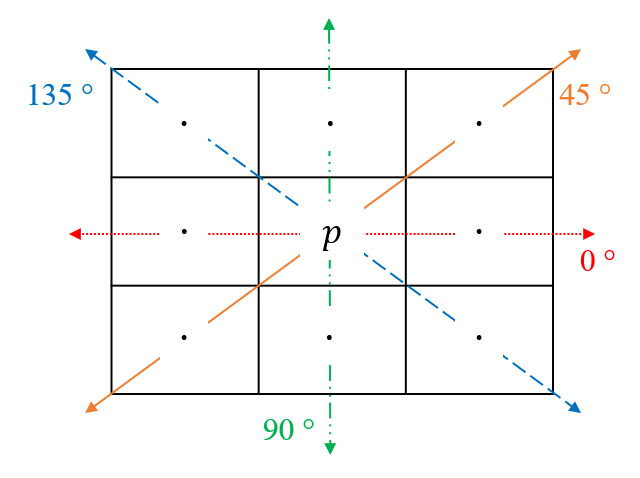
\includegraphics[width=\linewidth]{direction_fig.PNG}
      \caption{If we consider a certain pixel $p$ from a certain grayscale image $A$, we can define the angle-dependent spatial relationships as shown. Each arrow represents the line on which we compute $d-$distance nearest neighbors from our pixel $p$. The red, dotted line shows the 0\textdegree  path; the orange, solid line shows 45\textdegree  path; the green, dotted and dashed line shows the 90\textdegree  path, and the blue, dashed line shows the 135\textdegree  path. Adapted from: Robert Haralick, K. Shanmugam, and Ih Dinstein. Textural features for image classification. \textit{IEEE Trans Syst Man Cybern}, SMC-3:610–621, 01 1973. }
      \label{fig:directions}
    \end{figure}
    
\subsection{MPI}
   
\section{Related Work}

\section{Parallel Algorithm}

\section{Experimental Results}
\subsection{Simulated Experiments}
\subsection{Cluster Experiments}

\section{Conclusion }

\bibliography{references}

% The style file uses the \texttt{hyperref} package to make clickable
% links in documents. If this causes problems for you, add
% \texttt{nohyperref} as one of the options to the \texttt{icml2021}
% usepackage statement.





% \begin{figure}[ht]
% \vskip 0.2in
% \begin{center}
% \centerline{\includegraphics[width=\columnwidth]{icml_numpapers}}
% \caption{Historical locations and number of accepted papers for International
% Machine Learning Conferences (ICML 1993 -- ICML 2008) and International
% Workshops on Machine Learning (ML 1988 -- ML 1992). At the time this figure was
% produced, the number of accepted papers for ICML 2008 was unknown and instead
% estimated.}
% \label{icml-historical}
% \end{center}
% \vskip -0.2in
% \end{figure}

% \subsection{Figures}

% You may want to include figures in the paper to illustrate
% your approach and results. Such artwork should be centered,
% legible, and separated from the text. Lines should be dark and at
% least 0.5~points thick for purposes of reproduction, and text should
% not appear on a gray background.

% Label all distinct components of each figure. If the figure takes the
% form of a graph, then give a name for each axis and include a legend
% that briefly describes each curve. Do not include a title inside the
% figure; instead, the caption should serve this function.

% Number figures sequentially, placing the figure number and caption
% \emph{after} the graphics, with at least 0.1~inches of space before
% the caption and 0.1~inches after it, as in
% Figure~\ref{icml-historical}. The figure caption should be set in
% 9~point type and centered unless it runs two or more lines, in which
% case it should be flush left. You may float figures to the top or
% bottom of a column, and you may set wide figures across both columns
% (use the environment \texttt{figure*} in \LaTeX). Always place
% two-column figures at the top or bottom of the page.

% \subsection{Citations and References}

% Please use APA reference format regardless of your formatter
% or word processor. If you rely on the \LaTeX\/ bibliographic
% facility, use \texttt{natbib.sty} and \texttt{icml2021.bst}
% included in the style-file package to obtain this format.

% Citations within the text should include the authors' last names and
% year. If the authors' names are included in the sentence, place only
% the year in parentheses, for example when referencing Arthur Samuel's
% pioneering work \yrcite{Samuel59}. Otherwise place the entire
% reference in parentheses with the authors and year separated by a
% comma \cite{Samuel59}. List multiple references separated by
% semicolons \cite{kearns89,Samuel59,mitchell80}. Use the `et~al.'
% construct only for citations with three or more authors or after
% listing all authors to a publication in an earlier reference \cite{MachineLearningI}.

% Authors should cite their own work in the third person
% in the initial version of their paper submitted for blind review.
% Please refer to Section~\ref{author info} for detailed instructions on how to
% cite your own papers.

% Use an unnumbered first-level section heading for the references, and use a
% hanging indent style, with the first line of the reference flush against the
% left margin and subsequent lines indented by 10 points. The references at the
% end of this document give examples for journal articles \cite{Samuel59},
% conference publications \cite{langley00}, book chapters \cite{Newell81}, books
% \cite{DudaHart2nd}, edited volumes \cite{MachineLearningI}, technical reports
% \cite{mitchell80}, and dissertations \cite{kearns89}.

% Alphabetize references by the surnames of the first authors, with
% single author entries preceding multiple author entries. Order
% references for the same authors by year of publication, with the
% earliest first. Make sure that each reference includes all relevant
% information (e.g., page numbers).

% Please put some effort into making references complete, presentable, and
% consistent. If using bibtex, please protect capital letters of names and
% abbreviations in titles, for example, use \{B\}ayesian or \{L\}ipschitz
% in your .bib file.

% \section*{Software and Data}

% If a paper is accepted, we strongly encourage the publication of software and data with the
% camera-ready version of the paper whenever appropriate. This can be
% done by including a URL in the camera-ready copy. However, \textbf{do not}
% include URLs that reveal your institution or identity in your
% submission for review. Instead, provide an anonymous URL or upload
% the material as ``Supplementary Material'' into the CMT reviewing
% system. Note that reviewers are not required to look at this material
% when writing their review.

% % Acknowledgements should only appear in the accepted version.
% \section*{Acknowledgements}

% \textbf{Do not} include acknowledgements in the initial version of
% the paper submitted for blind review.

% If a paper is accepted, the final camera-ready version can (and
% probably should) include acknowledgements. In this case, please
% place such acknowledgements in an unnumbered section at the
% end of the paper. Typically, this will include thanks to reviewers
% who gave useful comments, to colleagues who contributed to the ideas,
% and to funding agencies and corporate sponsors that provided financial
% support.


% % In the unusual situation where you want a paper to appear in the
% % references without citing it in the main text, use \nocite
% \nocite{langley00}

% \bibliography{example_paper}
% \bibliographystyle{icml2021}


% %%%%%%%%%%%%%%%%%%%%%%%%%%%%%%%%%%%%%%%%%%%%%%%%%%%%%%%%%%%%%%%%%%%%%%%%%%%%%%%
% %%%%%%%%%%%%%%%%%%%%%%%%%%%%%%%%%%%%%%%%%%%%%%%%%%%%%%%%%%%%%%%%%%%%%%%%%%%%%%%
% % DELETE THIS PART. DO NOT PLACE CONTENT AFTER THE REFERENCES!
% %%%%%%%%%%%%%%%%%%%%%%%%%%%%%%%%%%%%%%%%%%%%%%%%%%%%%%%%%%%%%%%%%%%%%%%%%%%%%%%
% %%%%%%%%%%%%%%%%%%%%%%%%%%%%%%%%%%%%%%%%%%%%%%%%%%%%%%%%%%%%%%%%%%%%%%%%%%%%%%%
% \appendix
% \section{Do \emph{not} have an appendix here}

% \textbf{\emph{Do not put content after the references.}}
% %
% Put anything that you might normally include after the references in a separate
% supplementary file.

% We recommend that you build supplementary material in a separate document.
% If you must create one PDF and cut it up, please be careful to use a tool that
% doesn't alter the margins, and that doesn't aggressively rewrite the PDF file.
% pdftk usually works fine. 

% \textbf{Please do not use Apple's preview to cut off supplementary material.} In
% previous years it has altered margins, and created headaches at the camera-ready
% stage. 
% %%%%%%%%%%%%%%%%%%%%%%%%%%%%%%%%%%%%%%%%%%%%%%%%%%%%%%%%%%%%%%%%%%%%%%%%%%%%%%%
% %%%%%%%%%%%%%%%%%%%%%%%%%%%%%%%%%%%%%%%%%%%%%%%%%%%%%%%%%%%%%%%%%%%%%%%%%%%%%%%


\end{document}


% This document was modified from the file originally made available by
% Pat Langley and Andrea Danyluk for ICML-2K. This version was created
% by Iain Murray in 2018, and modified by Alexandre Bouchard in
% 2019 and 2021. Previous contributors include Dan Roy, Lise Getoor and Tobias
% Scheffer, which was slightly modified from the 2010 version by
% Thorsten Joachims & Johannes Fuernkranz, slightly modified from the
% 2009 version by Kiri Wagstaff and Sam Roweis's 2008 version, which is
% slightly modified from Prasad Tadepalli's 2007 version which is a
% lightly changed version of the previous year's version by Andrew
% Moore, which was in turn edited from those of Kristian Kersting and
% Codrina Lauth. Alex Smola contributed to the algorithmic style files.